\documentclass[icelandic]{beamer}

\mode<presentation>  % handout
{
  \usetheme[default]{Singapore}
  \usecolortheme{default}
  \usefonttheme{default}
  \setbeamertemplate{navigation symbols}{}
  \setbeamertemplate{caption}[numbered]
}

\usepackage{ucs}
\usepackage[utf8x]{inputenc}
\usepackage[english, icelandic]{babel}
\usepackage{t1enc}

\usepackage{xargs}
\usepackage{amsmath,amsthm}
\usepackage{mathtools,mathabx}
\usepackage{stmaryrd}
\newtheorem*{skilgreining}{Skilgreining}
\newtheorem*{daemi}{Dæmi}
\newtheorem*{spurning}{Spurning}

\usepackage{tilings}

%%%%%%%%%%% MACROS FOR DRAWING INTERVAL AND MESH PATTERNS %%%%%%%%%%%

\usepackage{tikz}
\usetikzlibrary{patterns}

% Sub-macros
\newcommand{\shadetheboxesPM}[1]{
    \foreach \x/\y in {#1}
    \fill[pattern color = black!75, pattern=north east lines] (\x,\y) rectangle +(1,1);
}

\newcommand{\drawthegrid}[1]{
    \draw (0.01,0.01) grid (#1+0.99,#1+0.99);
}

\newcommand{\drawverticallines}[3]{
    \foreach \x in {#2}
    \draw[line width=#3] (\x+0.01,0.01) -- (\x+0.01,#1+0.99);
}

\newcommand{\drawhorizontallines}[3]{
    \foreach \y in {#2}
    \draw[line width=#3] (0.01,\y+0.01) -- (#1+0.99,\y+0.01);
}

\newcommand{\drawtheclpattern}[1]{
    \foreach \x/\y in {#1}
    \filldraw (\x,\y) circle (6pt);
}

\newcommand{\drawclpattern}[2]{
	\foreach[count=\x] \y in {#1}
	{
		\filldraw (\x,\y) circle (#2 pt);
	}
}

\newcommand{\drawspecialbox}[1]{
    \foreach \x/\y/\z/\w/\A in {#1}
    {
        \fill[color = white!100, opacity=1, rounded corners = 1.5pt] (\x+0.125,\y+0.125) rectangle (\z-0.125,\w-0.125);
        \draw[color = black, rounded corners = 1.5pt] (\x+0.125,\y+0.125) rectangle (\z-0.125,\w-0.125);
        \fill[black] (\x/2+\z/2,\y/2+\w/2) node {\A};
    }
}

\newcommand{\drawspecialboxlarge}[1]{
    \foreach \x/\y/\z/\w/\A in {#1}
    {
        \fill[color = white!100, opacity=1, rounded corners = 1.5pt] (\x+0.125,\y+0.125) rectangle (\z-0.125,\w-0.125);
        \draw[color = black, rounded corners = 1.5pt] (\x+0.125,\y+0.125) rectangle (\z-0.125,\w-0.125);
        \fill[black] (\x/2+\z/2,\y/2+\w/2) node {\Large \A};
    }
}

\newcommand{\drawsolidshadedbox}[1]{
    \foreach \x/\y/\z/\w/\A in {#1}
    {
        \fill[color = gray!50, opacity=1, rounded corners=1.5pt] (\x+0.125,\y+0.125) rectangle (\z-0.125,\w-0.125);
        \draw[color = black, rounded corners=1.5pt] (\x+0.125,\y+0.125) rectangle (\z-0.125,\w-0.125);
        \fill[black] (\x/2+\z/2,\y/2+\w/2) node {\A};
    }
}

\newcommand{\drawlabels}[1]{
	\foreach \x/\y/\lab in {#1}
	{
		\draw (\x + 0.5,\y + 0.5) node {\lab};
	}
}


\newcommand{\pOneTwo}[1]{\mbox{\patt{#1}{2}{1,2}[][][][][][7]}}
\newcommand{\pTwoOne}[1]{\mbox{\patt{#1}{2}{2,1}[][][][][][7]}}
\newcommand{\pOneTwoThree}[1]{\mbox{\patt{#1}{3}{1,2,3}[][][][][][7]}}
\newcommand{\pOneThreeTwo}[1]{\mbox{\patt{#1}{3}{1,3,2}[][][][][][7]}}
\newcommand{\pTwoOneThree}[1]{\mbox{\patt{#1}{3}{2,1,3}[][][][][][7]}}
\newcommand{\pOneThreeTwoFour}[1]{\mbox{\patt{#1}{4}{1,3,2,4}[][][][][][7]}}

\newcommand{\etcdots}[2]{
	\scalebox{#1}
	{
		\begin{tikzpicture}[baseline=(current bounding box.center)]
			\filldraw (0,2) circle (#2 pt);
			\filldraw (1,1) circle (#2 pt);
			\filldraw (2,0) circle (#2 pt);
		\end{tikzpicture}
	}
}

\newcommand{\etcdotsflipped}[2]{
    \scalebox{#1}
    {
        \begin{tikzpicture}[baseline=(current bounding box.center)]
            \filldraw (0,0) circle (#2 pt);
            \filldraw (1,1) circle (#2 pt);
            \filldraw (2,2) circle (#2 pt);
        \end{tikzpicture}
    }
}

\newcommand{\decr}{\etcdots{0.2}{6}}
\newcommand{\incr}{\etcdotsflipped{0.2}{6}}


% #1: Scale
% #2: Length
% #3: Points
% #4: Shades
% #5: Markings
% #6: Avoidance decorations
% #7: Containment decorations
% #8: Labels
% #9: Size of the points
\newcommand{\patt}[9][4={},5={},6={},7={},8={},9=4]
{
	\scalebox{#1}
	{
		\begin{tikzpicture}[baseline=(current bounding box.center)]
			\useasboundingbox (0.0,-.3) rectangle (#2+1,#2+1.3);
			\shadetheboxesPM{#4}
			\draw (0.01,0.01) grid (#2+1-0.01,#2+1-0.01);

			\drawsolidshadedbox{#6}
			\drawspecialbox{#7}
			\drawspecialboxlarge{#5}
			\drawclpattern{#3}{#9}
			\drawlabels{#8}
		\end{tikzpicture}
	}
}

% #1: Scale
% #2: Length
% #3: Points
% #4: Shades
% #5: Markings
% #6: Avoidance decorations
% #7: Containment decorations
% #8: Circled points
\newcommand{\cpatt}[8][4={},5={},6={},7={},8={}]
{
	\scalebox{#1}
	{
		\begin{tikzpicture}[baseline=(current bounding box.center)]
			\useasboundingbox (0.0,-.3) rectangle (#2+1,#2+1.3);
			\shadetheboxesPM{#4}
			\draw (0.01,0.01) grid (#2+1-0.01,#2+1-0.01);

			\drawsolidshadedbox{#6}
			\drawspecialbox{#7}
			\drawspecialboxlarge{#5}
			\drawclpattern{#3}{4}

			\foreach \x/\y in {#8}
			{
				\draw[line width=1] (\x,\y) circle (7 pt);
			}
		\end{tikzpicture}
	}
}


% #1: Scale
% #2: Width/Height
% #3: Pattern lines
% #4: Added lines
% #5: Points
% #6: Shadings
% #7: Markings
% #8: Ascending restrictions
\newcommand{\metapatt}[8][6={},7={},8={}]
{
    \scalebox{#1}
    {
        \begin{tikzpicture}[baseline=(current bounding box.center)]
					\foreach \width/\height in {#2}
					{
						\useasboundingbox (0.0,-.3) rectangle (\width+1,\height+1.3);
            \shadetheboxesPM{#6}

            \foreach \pos/\type in {#4}
            {
                \ifthenelse{\equal{\type}{v}}
                {
                    \drawverticallines{\height}{\pos}{1.7pt}
                }
                {
								    \ifthenelse{\equal{\type}{d}}
                    {
                      \draw[densely dashed] (\pos,0) -- (\pos,\height+1);
                    }
										{
											\drawhorizontallines{\width}{\pos}{1.7pt}
										}
                }
            }

            \foreach \pos/\type in {#3}
            {
                \ifthenelse{\equal{\type}{v}}
                {
                    \drawverticallines{\height}{\pos}{0.6pt}
                }
                {
										\drawhorizontallines{\width}{\pos}{0.6pt}
                }
            }

            \drawsolidshadedbox{#8}
            \drawspecialbox{#7}

            \foreach \x/\y/\type in {#5}
            {
                \ifthenelse{\equal{\type}{a}}
                {
                    % Added point
                    \draw (\x,\y) circle (6pt);
                    \filldraw (\x,\y) circle (3pt);
                }
                {
                    % Pattern point
                    \filldraw (\x,\y) circle (4pt);
                }
            }
					}
        \end{tikzpicture}
    }
}

% #1: Scale
% #2: Width/Height
% #3: Pattern lines
% #4: Added lines
% #5: Points
% #6: Shadings
% #7: Markings
% #8: Ascending restrictions
% #9: Labels
\newcommand{\dpatt}[9][6={},7={},8={},9={}]
{
    \scalebox{#1}
    {
        \begin{tikzpicture}[baseline=(current bounding box.center)]
					\foreach \width/\height in {#2}
					{
						\useasboundingbox (0.0,-.3) rectangle (\width+1,\height+1.3);
            \shadetheboxesPM{#6}

            \foreach \pos/\type in {#4}
            {
                \ifthenelse{\equal{\type}{v}}
                {
                    \drawverticallines{\height}{\pos}{1.7pt}
                }
                {
								    \ifthenelse{\equal{\type}{d}}
                    {
                      \draw[densely dashed] (\pos,0) -- (\pos,\height+1);
                    }
										{
											\drawhorizontallines{\width}{\pos}{1.7pt}
										}
                }
            }

            \foreach \pos/\type in {#3}
            {
                \ifthenelse{\equal{\type}{v}}
                {
                    \drawverticallines{\height}{\pos}{0.6pt}
                }
                {
										\drawhorizontallines{\width}{\pos}{0.6pt}
                }
            }

            \drawsolidshadedbox{#8}
            \drawspecialbox{#7}

            \foreach \x/\y/\type in {#5}
            {
                \ifthenelse{\equal{\type}{a}}
                {
                    % Added point
                    \draw9 (\x,\y) circle (6pt);
                    \filldraw (\x,\y) circle (3pt);
                }
                {
                    % Pattern point
                    \filldraw (\x,\y) circle (4pt);
                }
            }

						\drawlabels{#9}
					}
        \end{tikzpicture}
    }
}

\newcommand{\mpattern}[4]{										% mesh pattern for text
  \raisebox{0.6ex}{
  \begin{tikzpicture}[scale=0.35, baseline=(current bounding box.center), #1]
  	\useasboundingbox (0.0,-0.1) rectangle (#2+1.4,#2+1.1);

    \shadetheboxesPM{#4}

    \drawthegrid{#2}

    \drawtheclpattern{#3}

  \end{tikzpicture}}
}

% FROM TSA

\newcommand{\textmpattern}[4]{                                      % mesh pattern for text
    \scalebox{#1}
    {
      \begin{tikzpicture}[baseline=(current bounding box.center)]
        \useasboundingbox (0.0,0) rectangle (#2+1,#2+0);
        \shadetheboxesPM{#4}

        \drawthegrid{#2}

        \drawclpattern{#3}{6}

      \end{tikzpicture}
    }
}


% #1: Scale
% #2: Length
% #3: Points
% #4: Shades
% #5: Circled points
% #6: Added lines
% #7: Arrows
\newcommandx{\shpatt}[7][4={},5={},6={},7={}]
{
    \scalebox{#1}
    {
        \begin{tikzpicture}[baseline=(current bounding box.center)]
            \useasboundingbox (0.0,-.3) rectangle (#2+1,#2+1);
            \shadetheboxesPM{#4}
            \draw (0.01,0.01) grid (#2+1-0.01,#2+1-0.01);

            \drawclpattern{#3}{4}

            \foreach \x/\y in {#5}
            {
                \draw[line width=1] (\x,\y) circle (7 pt);
            }

            \foreach \x/\y in {#6}
            {
                \draw[densely dashed, line width=1.7pt] (\x,0) -- (\x,#2+1);
                \draw[densely dashed, line width=1.7pt] (0,\y) -- (#2+1,\y);
            }

            \foreach \xa/\ya/\xb/\yb in {#7}
            {
                \draw[->, line width=1.7pt] (\xa,\ya) -- (\xb-0.12,\yb-0.12);
            }
        \end{tikzpicture}
    }
}

% #1: Scale
% #2: Length
% #3: Points
% #4: Shades
% #5: Circled points
% #6: Added lines
% #7: Arrows
% #8: Special boxes
\newcommandx{\shpattb}[8][4={},5={},6={},7={},8={}]
{
    \scalebox{#1}
    {
        \begin{tikzpicture}[baseline=(current bounding box.center)]
            \useasboundingbox (0.0,-.3) rectangle (#2+1,#2+1);
            \shadetheboxesPM{#4}
            \draw (0.01,0.01) grid (#2+1-0.01,#2+1-0.01);

            \drawclpattern{#3}{4}

            \foreach \x/\y in {#5}
            {
                \draw[line width=1] (\x,\y) circle (7 pt);
            }

            \foreach \x/\y in {#6}
            {
                \draw[densely dashed, line width=1.7pt] (\x,0) -- (\x,#2+1);
                \draw[densely dashed, line width=1.7pt] (0,\y) -- (#2+1,\y);
            }

            \foreach \xa/\ya/\xb/\yb in {#7}
            {
                \draw[->, line width=1.7pt] (\xa,\ya) -- (\xb-0.12,\yb-0.12);
            }
            \foreach \xa/\ya/\xb/\yb in {#8}
            {
                \draw[line width=1.5pt] (\xa+0.1,\ya+0.1) rectangle (\xb-0.1,\yb-0.1);
            }
        \end{tikzpicture}
    }
}

\pgfmathsetmacro{\patttablescale}{1.05}
\pgfmathsetmacro{\pattdispscale}{0.80}
\pgfmathsetmacro{\patttextscale}{0.6}
\pgfmathsetmacro{\patttbeamerscale}{0.3}

\newcommand{\mb}[1]{{\mathbb{#1}}}
\newcommand{\mc}[1]{{\mathcal{#1}}}
\newcommand{\mf}[1]{{\mathfrak{#1}}}
\newcommand{\mr}[1]{{\mathrm{#1}}}

\renewcommand{\S}{\mathfrak{S}}
\newcommand{\Av}{\mathrm{Av}}
\newcommand{\Co}{\mathrm{Co}}
\newcommand{\st}{\mathrm{st}}
\newcommand{\Gr}{\mathrm{Gr}}
\newcommand{\Grid}{\mathrm{Grid}}
\newcommand{\Struct}{\textsf{Struct}}
\newcommand{\CombCov}{\textsf{CombCov}}
\newcommand{\CombSpecSearcher}{\textsf{CombSpecSearcher}}
\newcommand{\boks}[1]{{\lcorners{#1}\rcorners}}
\newcommand{\mediumsqcup}{\textstyle\bigsqcup}



\logo{\includegraphics[height=1.5cm]{RU_logo_transparent.png}}

\title[Fléttufræðilegar þakningar]{Þakningar fléttufræðilegra fyrirbrigða með aðstoð línulegrar bestunnar}
\subtitle{Stærðfræði á Íslandi 2019}
\author[Bjarni Jens, Christian og Henning]{\underline{Bjarni Jens Kristinsson}, Christian Bean og Henning Úlfarsson}
\institute{Háskólinn í Reykjavík}
\date{13.\@ október 2019}



\begin{document}

\begin{frame}\titlepage\end{frame}
\begin{frame}\tableofcontents\end{frame}


%%%%%%%%%%%%%%%%%%%%%%%%%%%%%%%%%%%%%%%%%%%%%%%%%%%%%%%%%%%%%%%%%%%%%%%%%%%%%%%
\section{Inngangur}
\subsection{Okkar framlag}
\begin{frame}{Bakgrunnur}
  \begin{itemize}
    \item M.Sc.\@ verkefni í tölvunarfræði við Háskólann í Reykjavík
    \item Byggir á \emph{,,Automatic discovery of structural rules of permutation classes``} (2019) eftir Christian Bean, Bjarka Guðmundsson og Henning Úlfarsson
    \item \Struct\ einskorðast við umraðanaklasa
  \end{itemize}
\end{frame}

\begin{frame}{Okkar framlag}
\begin{itemize}
  \item \CombCov\ hugbúnaðarpakka fyrir Python
  \item Almennt tól fyrir fléttufræðileg fyrirbrigði
  \item Sjálfvirknivætt eldri niðurstöður um möskvamynstursklasa
\end{itemize}
\end{frame}


%%%%%%%%%%%%%%%%%%%%%%%%%%%%%%%%%%%%%%%%%%%%%%%%%%%%%%%%%%%%%%%%%%%%%%%%%%%%%%%
\subsection{Orðaklasar}
\begin{frame}{Dæmi um fléttufræðilegt fyrirbrigði -- \emph{orðaklasar}}
  \uncover<1->{
    \begin{skilgreining}
      Látum $s$ vera orð með bókstöfum úr stafrófinu $\Sigma = \left\{ a,b \right\}$.
      Við táknum tóma orðið með $\epsilon$ og það uppfyllir skilyrðin $\epsilon \cdot s = s$
      (forskeyti) og $s \cdot \epsilon = s$ (viðskeyti) fyrir öll orð $s$ yfir $\Sigma$. 
      
      Skilgreinum $\Av(s)$ sem mengið af orðum yfir stafrófið $\Sigma$ sem innihalda
      ekki $s$ sem hlutorð. Köllum þetta \emph{orðaklasa}.
    \end{skilgreining}}
  \uncover<2->{
    \begin{daemi}
      \begin{itemize}
        \item<2-> $\Av(aa) = \left\{ \epsilon, a, b, ab, ba, bb, aba, abb, bab, bba, bbb, \ldots \right\}$ 
          er orðaklasi.
        \item<3->{Er til einfaldari lýsing á $\Av(aa)$?}
        \item<4->{Hvað eru mörg orð af lengd $n$ í $\Av(aa)$?}
      \end{itemize}
    \end{daemi}}
\end{frame}


%%%%%%%%%%%%%%%%%%%%%%%%%%%%%%%%%%%%%%%%%%%%%%%%%%%%%%%%%%%%%%%%%%%%%%%%%%%%%%%
\section{\CombCov\ reikniritið}
\subsection{Útskýring með orðaklösum}
\begin{frame}{Hugmyndin bak við \CombCov}
  \begin{itemize}[<+->]
    \item \underline{Markmið:} Finna $k$ sundurlæg hlutmengi $S_i$ sem \emph{þekja} $\Av(S)$
    \begin{enumerate}[(1)]
      \item $\bigcup_{i \in I}{S_i} = \Av(S)$
      \item $S_i \cap S_j = \emptyset$ ef $i \neq j$
    \end{enumerate}
    \item Köllum $\Av(S)$ \emph{rótina} og $S_i$ \emph{reglur}
    \item \underline{Vandamál:} Tölvur kunna ekki að reikna með óendanlega mörgum hlutum
    \item \underline{Lausn:} Búum til og vinnum með \emph{endanlegar} framsetningar
    \begin{itemize}
      \item $R = \left \{ w \in \Av(S) \colon |w| \leq \ell \right \}$
      \item $R_i = \left \{ w \in S_i \colon |w| \leq \ell \right \}$
    \end{itemize}
    \item Leysum í staðinn endanlega vandamálið
    \begin{enumerate}[(1)]
      \item $\bigcup_{i \in I}{R_i} = R$
      \item $R_i \cap R_j = \emptyset$ ef $i \neq j$
    \end{enumerate}
    \item Á næstu glærum förum við í gegn um reikniritið til að finna þakningu á $\Av(aa)$
  \end{itemize}
\end{frame}

\begin{frame}{Reglur}
  \begin{itemize}[<+->]
    \item $\Av(aa) = \left\{ \epsilon, a, b, ab, ba, bb, aba, abb, bab, bba, bbb, \ldots \right\}$
    \item Hvernig finnum við reglurnar $S_i$?
    \item Okkar hugmynd: Prófum reglur af gerðinni $u \Av(S')$ þar sem
      \begin{itemize}
        \item $u$ er orð í $\Av(S)$ að lengd $\leq \max \left \{ |w| \colon w \in S \right\}$ og 
        \item $S'$ er annað hvort allt stafrófið $\Sigma$ eða mengi af orðum sem eru hlutorð af orðum í $\Av(S)$
      \end{itemize}
    \item Næsta skref: Kanna hvort reglurnar séu \emph{gjaldgengar}
  \end{itemize}
\end{frame}

\begin{frame}{Bitastrengir}
  \begin{itemize}[<+->]
    \item $\Av(aa) = \left\{ \epsilon, a, b, ab, ba, bb, aba, abb, bab, bba, bbb, \ldots \right\}$
    \item Veljum nákvæmnina $\ell = 2$
    \item Þá er $R = \left \{ \epsilon, a, b, ab, ba, bb \right \}$
    \item Notum \emph{bitastrengi} til að tákna hlutmengi í $R$
      \begin{itemize}
        \item $B' = 111111$ táknar allt mengið $R$
        \item $B'' = 011001$ táknar hlutmengið $\{a, b, bb\}$
        \item $B''' = 100000$ táknar hlutmengið $\{\epsilon\}$
      \end{itemize}
    \item Reglan $a \Av(a)$ býr til mengið $R' = \{ a, ab \} \subseteq R$ með tilsvarandi bitastreng $010100$ og er því gjaldgeng
    \item Reglan $a \Av(b)$ býr til mengið $R'' = \{ a, aa \} \not \subseteq R$ svo reglan er ógjaldgeng
  \end{itemize}
\end{frame}

\begin{frame}{Línuleg bestun}
  \begin{itemize}[<+->]
    \item $R = \left \{ \epsilon, a, b, ab, ba, bb \right \}$
    \item Samtals verða til 16 reglur
      \begin{itemize}
        \item Þar af eru 15 gjaldgengar
        \item Þær búa til 9 ólíka bitastrengi
      \end{itemize}
    \item Notum \emph{Gurobi} eða \emph{COIN CLP/CBC LP} til að leysa jöfnuhneppið 
        \begin{alignat*}{17}
          \text{Min}    \qquad  & \mathrlap{z = x_1 + \cdots + x_9} & & & & & & & & & & & & & & & \\
          \text{þ.a.}   \qquad  & &     &     &     &     &     &     &     &     &     &     & x_6 &     &     & +{} & x_8 & +{} & x_9 & ={}  &  1 \\
                                & & x_1 &     &     &     &     &     &     &     &     &     &     &     &     &     &     &     &     & ={}  &  1 \\
                                & &     &     & x_2 &     &     &     &     &     &     &     &     & +{} & x_7 &     &     &     &     & ={}  &  1 \\
                                & &     &     &     &     & x_3 &     &     &     &     &     &     &     &     & +{} & x_8 & +{} & x_9 & ={}  &  1 \\
                                & &     &     &     &     &     &     & x_4 &     &     &     &     & +{} & x_7 &     &     &     &     & ={}  &  1 \\
                                & &     &     &     &     &     &     &     &     & x_5 &     &     &     &     &     &     & +{} & x_9 & ={}  &  1 \\
          \text{m.t.t.} \qquad  & \mathrlap{x_i \in \left\{ 0, 1 \right\} \text{ fyrir } i = 1, \ldots, 9.} & & & & & & & & & & & & & & &
      \end{alignat*}
  \end{itemize}
\end{frame}

\begin{frame}{Þakning $\Av(aa)$}
\begin{itemize}[<+->]
  \item Ein lausn jöfnuhneppisins er $x_1 = x_7 = x_9 = 1$ og gefur þakninguna \[ \epsilon \Av(a,b) \cup a \Av(a) \cup b \Av(aa) .\]
  \item Þetta er \emph{röng} lausn!
  \item $abba \in \Av(aa)$ en engin af reglunum býr til orðið!
  \item Með því að hækka nákæmnina (gildið á $\ell$) fæst rétt svar: \[\Av(aa) = \epsilon \Av(a,b) \cup a \Av(a,b) \cup b \Av(aa) \cup ab \Av(aa)\]
  \item Hægt er að sýna fram á að \emph{talning} orðaklasans séu Fibonacci tölurnar (hliðraðar um einn)
\end{itemize}
\end{frame}


%%%%%%%%%%%%%%%%%%%%%%%%%%%%%%%%%%%%%%%%%%%%%%%%%%%%%%%%%%%%%%%%%%%%%%%%%%%%%%%
\section{Umraðanir og möskvamynstur}
\subsection{Skilgreiningar}
\begin{frame}{Okkar viðfangsefni}
\begin{center}
  $\Av \left( \mpattern{scale=\patttablescale}{ 4 }{ 1/1, 2/3, 3/4, 4/2}{},
              \mpattern{scale=\patttablescale}{ 3 }{ 1/2, 2/3, 3/1 }{1/0,1/1,1/2,1/3, 0/1,2/1,3/1} \right)$
\end{center}
\end{frame}

\begin{frame}{Umraðanir}
    \uncover<1->{\emph{Umröðun (e.\@ permutation) að lengd $n$} er gagntæk vörpun á $\llbracket 1, n \rrbracket = \left\{ 1, \ldots, n \right\}$.} 
    \uncover<2->{Dæmi um umröðun að lengd 4 er $\pi = 1342$} \uncover<3->{sem varpar $1 \mapsto 1$, $2 \mapsto 3$, $3 \mapsto 4$ og $4 \mapsto 2$.}
    \uncover<4->{Myndræn framsetning á umröðunum lítur svona út:
    
    \begin{figure}[htbp]
      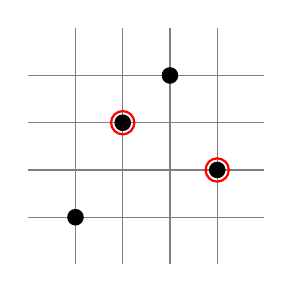
\begin{tikzpicture}[scale=.6, baseline={([yshift=-3pt]current bounding box.center)}]
        \def \n {4}
        \foreach \x in {1,...,\n} {
          \draw[gray] (0,\x) -- (\n+1,\x);
          \draw[gray] (\x,0) -- (\x,\n+1);
        }
        \foreach \x in {(1,1),(2,3),(3,4),(4,2)} {\fill[black] \x circle (5pt);}
        \uncover<5->{\foreach \x in {(2,3),(4,2)} {\draw[red, thick]  \x circle (7pt);}}
      \end{tikzpicture}
    \end{figure}}
  
    \uncover<5->{Við segjum að $\pi$ \emph{innihaldi} \emph{mynstrið} $p = 21$ því $32$ (í $1\underline{3}4\underline{2}$) er \emph{einsraða} (e.\@ \emph{order isomorphic}) $p$.}
    \uncover<6->{$\pi$ inniheldur ekki mynstrið $q = 312$ og þá segjum við að $\pi$ \emph{forðist} $q$.}
\end{frame}

\begin{frame}{Möskvamynstur}
    \begin{itemize}[<+->]
      \item \emph{Möskvamynstur (e.\@ mesh pattern)} er tvennd $\left( \pi, M \right)$ þar sem $\pi$ er umröðun að lengd $n$ og $M$ er hlutmengi í $\llbracket 0, n \rrbracket \times \llbracket 0, n \rrbracket$.
      \item Dæmi: $p = \left( 213, \left\{ \boks{1,2}, \boks{2,2}, \boks{2,3} \right\} \right)$
        \begin{figure}[h]
          \centering
          \mpattern{scale=\patttablescale}{ 3 }{ 1/2, 2/1, 3/3 }{ 1/2, 2/2, 2/3 }
        \end{figure}
    \end{itemize}
\end{frame}

\begin{frame}{Umröðun inniheldur möskvamynstur}
\begin{figure}[h]
  \centering
  \raisebox{0.6ex}{%{{{
  \shpattb{0.5}{3}{2,1,3}[1/2,2/2,2/3][][][][1/2/2/3, 2/2/3/3, 2/3/3/4]}
  \quad\quad
  \raisebox{0.6ex}{%{{{
    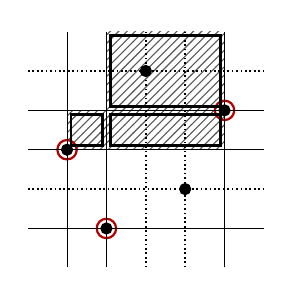
\begin{tikzpicture}[baseline=(current bounding box.center), scale=0.5]
      \useasboundingbox (0.0,-0.1) rectangle (5+1.4,5+1.1);
      \foreach \x/\y in {1/3,2/3,2/4,2/5,3/3,3/4,3/5,4/3,4/4,4/5}
        \fill[pattern color = black!65, pattern=north east lines] (\x,\y) rectangle +(1,1);
      \foreach [count=\x] \y in {3,1,5,2,4}
      \filldraw (\x,\y) circle (4pt);
      \foreach \x/\y in {1/3,2/1,5/4}
      \draw[thick,red!70!black] (\x,\y) circle (7pt);
      \draw[very thin] (1,0.01) -- (1,5.99);
      \draw[very thin] (2,0.01) -- (2,5.99);
      \draw[very thin] (5,0.01) -- (5,5.99);
      \draw[very thin] (0.01,1) -- (5.99,1);
      \draw[very thin] (0.01,3) -- (5.99,3);
      \draw[very thin] (0.01,4) -- (5.99,4);

      \draw[densely dotted, line width=0.6pt] (3,0.01) -- (3,5.99);
      \draw[densely dotted, line width=0.6pt] (4,0.01) -- (4,5.99);
      \draw[densely dotted, line width=0.6pt] (0.01,2) -- (5.99,2);
      \draw[densely dotted, line width=0.6pt] (0.01,5) -- (5.99,5);

      \foreach \xa/\ya/\xb/\yb in {1/3/2/4, 2/3/5/4, 2/4/5/6}
            {
              \draw[line width=1pt] (\xa+0.1,\ya+0.1) rectangle (\xb-0.1,\yb-0.1);
            }
    \end{tikzpicture}}%}}}
    \quad\quad
    \raisebox{0.6ex}{%{{{
    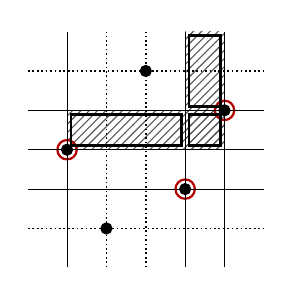
\begin{tikzpicture}[baseline=(current bounding box.center), scale=0.5]
      \useasboundingbox (0.0,-0.1) rectangle (5+1.4,5+1.1);
      \foreach \x/\y in {1/3,2/3,3/3,4/3,4/3,4/4,4/5}
        \fill[pattern color = black!65, pattern=north east lines] (\x,\y) rectangle +(1,1);
      \foreach [count=\x] \y in {3,1,5,2,4}
      \filldraw (\x,\y) circle (4pt);
      \foreach \x/\y in {1/3,4/2,5/4}
      \draw[thick,red!70!black] (\x,\y) circle (7pt);
      \draw[very thin] (1,0.01) -- (1,5.99);
      \draw[very thin] (4,0.01) -- (4,5.99);
      \draw[very thin] (5,0.01) -- (5,5.99);
      \draw[very thin] (0.01,2) -- (5.99,2);
      \draw[very thin] (0.01,3) -- (5.99,3);
      \draw[very thin] (0.01,4) -- (5.99,4);

      \draw[densely dotted, line width=0.6pt] (2,0.01) -- (2,5.99);
      \draw[densely dotted, line width=0.6pt] (3,0.01) -- (3,5.99);
      \draw[densely dotted, line width=0.6pt] (0.01,1) -- (5.99,1);
      \draw[densely dotted, line width=0.6pt] (0.01,5) -- (5.99,5);

        \foreach \xa/\ya/\xb/\yb in {1/3/4/4, 4/3/5/4, 4/4/5/6}
            {
              \draw[line width=1pt] (\xa+0.1,\ya+0.1) rectangle (\xb-0.1,\yb-0.1);
            }
    \end{tikzpicture}}%}}}
    \end{figure}
    \begin{itemize}[<+->]
      \item Her að ofan sést dæmi um tilvik af möskvamynstrinu $p = \left( 213, \left\{ \boks{1,2}, \boks{2,2}, \boks{2,3} \right\} \right)$ í umröðuninni $\pi = 31524$.
      \item Mengi allra umraðana sem \emph{forðast} möskvamynstrið $p$ er $\Av(p)$.
      \item Mengi allra umraðana \emph{af lengd} $n$ sem forðast $p$ er $\Av_n(p)$.
      \item \emph{Talning} möskvamynstursklasans $\Av(p)$ er talnaruna $(F_n)_{n = 0}^{+\infty}$ þ.a.\@ $|\Av_n(p)| = F_n$.
      \item Summan $\Sigma_{n = 0}^{+\infty} F_n x^n$ er \emph{framleiðnifall} möskvamynstursklasans $\Av(p)$.
    \end{itemize}
\end{frame}


%%%%%%%%%%%%%%%%%%%%%%%%%%%%%%%%%%%%%%%%%%%%%%%%%%%%%%%%%%%%%%%%%%%%%%%%%%%%%%%
\subsection{Áhugaverðar niðurstöður}
\begin{frame}{Áhugaverðar niðurstöður}\center{Næst skoðum við nokkrar áhugaverðar niðurstöður.}\end{frame}
\begin{frame}{\emph{Enumerations of Permutations Simultaneously Avoiding a Vincular and a Covincular Pattern of Length 3} (2017)}
\begin{figure}[h]
  \centering
  \begin{tabular}{ r c l l }
    $\Av \left( \mpattern{scale=\patttextscale}{ 3 }{ 1/1, 2/2, 3/3 }{ 1/0, 1/1, 1/2, 1/3 }, \mpattern{scale=\patttextscale}{ 3 }{ 1/2, 2/1, 3/3 }{0/2, 1/2, 2/2, 3/2 } \right)$ & $=$ & $
    \strule{\patttextscale}{1}{1}{} \mediumsqcup
    \strule{\patttextscale}{2}{2}{
      (0,1)/$\mc{A}$, 
      (1,0)/\point{2pt}
    } \mediumsqcup
    \strule{\patttextscale}{4}{4}{
      (0,3)/$\mc{A}$, 
      (1,0)/\point{2pt},
      (2,2)/\point{2pt},
      (3,1)/$\mc{A}$
    } $ &
  \end{tabular}
\end{figure}

Af þessari þakningu sjáum við að um framleiðnifallið $F(X)$ gildir
\[ F(x) = 1 + xF(x) + x^2F(x)^2 \]
sem gefa okkur \emph{Motzkin} tölurnar $M_n$.
\end{frame}

\begin{frame}{\emph{Wilf-Classification of Mesh Patterns of Short Length} (2015)}
\begin{table}[h]
  \centering
  \begin{tabular}{ r c l l }
    $\Av \left( \mpattern{scale=\patttextscale}{ 2 }{ 1/2, 2/1 }{ 0/0, 0/1, 0/2, 1/0, 1/2, 2/0, 2/1 } \right)$ & $=$ & $
      \strule{\pattdispscale}{1}{1}{} \mediumsqcup
      \strule{\pattdispscale}{2}{2}{
        (0,0)/\point{2pt}, 
        (1,1)/$\mc{B}$
      } \mediumsqcup
      \strule{\pattdispscale}{2}{2}{
        (0,1)/\point{2pt}, 
        (1,0)/\point{2pt},
        (1,1)/$\S$
      }$ & \\
  $\Co \left( \mpattern{scale=\patttextscale}{ 2 }{ 1/2, 2/1 }{ 0/0, 0/1, 0/2, 1/0, 1/2, 2/0, 2/1 } \right)$ & $=$ & $
      \strule{\pattdispscale}{4}{4}{
        (0,0)/\point{2pt}, 
        (1,1)/$\S$,
        (2,2)/\point{2pt},
        (3,3)/$\mc{B}$
    }$ & $\mc{B} = \Av \left( \mpattern{scale=\patttextscale}{ 1 }{ 1/1 }{ 0/1, 1/0 } \right)$
  \end{tabular}
\end{table} 
\end{frame}

\begin{frame}
\begin{table}[h]
  \centering
  \begin{tabular}{ r c l l }
    $\Av \left( \mpattern{scale=\patttextscale}{ 2 }{ 1/2, 2/1 }{ 0/1, 0/2, 1/0, 1/2, 2/0, 2/1 } \right)$ & $=$ & $
    \strule{\pattdispscale}{1}{1}{
      (0,0)/$\mc{B}$
    } \mediumsqcup
    \strule{\pattdispscale}{3}{3}{
      (0,0)/$\mc{B}$, 
      (1,1)/\point{2pt},
      (2,2)/$\mc{B}$
    }$ & \\
    $\Co \left( \mpattern{scale=\patttextscale}{ 2 }{ 1/2, 2/1 }{ 0/1, 0/2, 1/0, 1/2, 2/0, 2/1 } \right)$ & $=$ & $ 
    \strule{\pattdispscale}{5}{5}{
      (0,0)/$\S$,
      (1,1)/\point{2pt}, 
      (2,2)/$\mc{B}$,
      (3,3)/\point{2pt},
      (4,4)/$\mc{B}$
    }$  & $\mc{B} = \Av \left( \mpattern{scale=\patttextscale}{ 1 }{ 1/1 }{ 0/1, 1/0 } \right)$
  \end{tabular}
\end{table} 
\end{frame}

\begin{frame}
\begin{table}[h]
  \centering
  \begin{tabular}{ r c l l }
    $\Co \left( \mpattern{scale=\patttextscale}{ 2 }{ 1/2, 2/1 }{ 0/0, 0/1, 1/1, 1/2, 2/0, 2/2 } \right)$ & $=$ & $
    \strule{\pattdispscale}{5}{5}{
      (0,4)/$\S$, 
      (1,1)/\point{2pt},
      (2,0)/$\S$,
      (3,3)/\point{2pt},
      (4,2)/$\S$
    }$ &
  \end{tabular}
\end{table} 
\end{frame}

\begin{frame}{\emph{Generalized Pattern Avoidance} (2001)}
\begin{table}[h]
  \centering
  \begin{tabular}{ r c l l }
    $\Av \left( \mpattern{scale=\patttextscale}{ 3 }{ 1/1, 2/2, 3/3 }{ 2/0, 2/1, 2/2, 2/3 } \right)$ & $=$ & $ 
    \strule{\pattdispscale}{1}{1}{} \mediumsqcup
    \strule{\pattdispscale}{3}{2}{
      (0,1)/$\mc{A}$,
      (1,0)/\point{2pt}, 
      (2,1)/$\mc{B}$
    }$ &  $\mc{A} = \Av \left( \mpattern{scale=\patttextscale}{ 3 }{ 1/1, 2/2, 3/3 }{ 2/0, 2/1, 2/2, 2/3 } \right)$ \\
    & & & $\mc{B} = \Av \left( \mpattern{scale=\patttextscale}{ 2 }{ 1/1, 2/2 }{} \right)$
  \end{tabular}
\end{table}

Hægt er að leiða út framleiðnifallið sem gæfi okkur \emph{Bell} tölurnar $B_n$.
\end{frame}

\begin{frame}{\emph{Wilf classification of bi-vincular permutation patterns} (2009)}
\begin{figure}[h]
  \centering
  \begin{tabular}{ r c l l }
    $\Av \left( \mpattern{scale=\patttextscale}{ 3 }{ 1/1, 2/3, 3/2 }{ 0/3, 1/3, 2/3, 3/3 } \right)$ & $=$ & $
    \strule{\pattdispscale}{1}{1}{} \mediumsqcup
    \strule{\pattdispscale}{3}{3}{
      (0,1)/$\S$,
      (1,2)/\point{2pt},
      (2,0)/$\S$
    }$ & \\
    \uncover<2->{
      $\Av \left( \mpattern{scale=\patttextscale}{ 3 }{ 1/1, 2/3, 3/2 }{} \right)$ & $=$ & $
      \strule{\pattdispscale}{1}{1}{} \mediumsqcup
      \strule{\pattdispscale}{3}{3}{
        (0,1)/$\mc{A}$,
        (1,2)/\point{2pt},
        (2,0)/$\mc{A}$
      }$ & $\mc{A} = \Av \left( \mpattern{scale=\patttextscale}{ 3 }{ 1/1, 2/3, 3/2 }{} \right)$
    }
  \end{tabular}
\end{figure}
\end{frame}


%%%%%%%%%%%%%%%%%%%%%%%%%%%%%%%%%%%%%%%%%%%%%%%%%%%%%%%%%%%%%%%%%%%%%%%%%%%%%%%
\section{Lokaorð og spurningar}
\begin{frame}
  \center{Einhverjar spurningar?}
\end{frame}

\end{document}
